\documentclass[aps,pre,twocolumn,showpacs,preprintnumbers,amsmath,amssymb]{revtex4-1}
%\documentclass[preprint,showpacs,preprintnumbers,amsmath,amssymb]{revtex4}

% Some other (several out of many) possibilities
%\documentclass[preprint,aps]{revtex4}
%\documentclass[preprint,aps,draft]{revtex4}
%\documentclass[prb]{revtex4}% Physical Review B

\usepackage{graphicx}% Include figure files
\usepackage{dcolumn}% Align table columns on decimal point
\usepackage{bm}% bold math

\usepackage[latin1]{inputenc}
\usepackage{amsfonts}
\usepackage{amsmath}
\usepackage{amssymb}
\usepackage{amsthm}
\usepackage{bbold}
\usepackage{color}
\usepackage[american]{babel}
\usepackage[T1]{fontenc}
\usepackage{longtable}
%\usepackage[dvips]{graphicx}
\usepackage{xspace}
\usepackage{bbm}
\usepackage[all]{xy}
%\usepackage{slashbox}
%\usepackage[justification=centering]{caption}
\providecommand{\begeq}[1]{\begin{equation}#1\end{equation}}
\DeclareMathOperator{\tr}{tr}
\providecommand{\norm}[1]{\lVert#1\rVert}
\newtheorem{theorem}{Theorem}
\newtheorem{lemma}{Lemma}
\newtheorem{defi}{Definition}
\newtheorem{rem}{Remark}
\newtheorem{conj}{Conjecture}
\newtheorem{prop}{Proposition}
\DeclareMathOperator{\con}{cond}
\DeclareMathOperator{\diag}{diag}
\newcolumntype{C}[1]{>{\centering\arraybackslash}p{#1}}

\begin{document}

%\preprint{APS/123-QED}

\title{TBD}% Force line breaks with \\

%\author{}
%\author{}
%\affiliation{
%}
%Lines break automatically or can be forced with \\

\author{Varadarajan Rengaraj}
\email{rengaraj@campus.uni-paderborn.de}
%\affiliation{Institute for Physical Chemistry and Center for Computational Sciences, Johannes Gutenberg University of Mainz, Staudinger Weg 7, D-55128 Mainz, Germany}
%\affiliation{
%Dynamics of Condensed Matter and Center for Sustainable Systems Design, Department of Chemistry, University of Paderborn, Warburger Str. 100, D-33098 Paderborn, Germany
%}
\affiliation{Department of Computer science, Paderborn University, Warburger Str. 100, D-33098 Paderborn, Germany}

\author{Michael Lass}
\email{michael.lass@uni-paderborn.de}
%\affiliation{Institute for Physical Chemistry and Center for Computational Sciences, Johannes Gutenberg University of Mainz, Staudinger Weg 7, D-55128 Mainz, Germany}
%\affiliation{
%Dynamics of Condensed Matter and Center for Sustainable Systems Design, Department of Chemistry, University of Paderborn, Warburger Str. 100, D-33098 Paderborn, Germany
%}
\affiliation{Department of Computer science, Paderborn University, Warburger Str. 100, D-33098 Paderborn, Germany}

\author{Christian Plessl}
\email{christian.plessl@uni-paderborn.de}
%\affiliation{Institute for Physical Chemistry and Center for Computational Sciences, Johannes Gutenberg University of Mainz, Staudinger Weg 7, D-55128 Mainz, Germany}
%\affiliation{
%Dynamics of Condensed Matter and Center for Sustainable Systems Design, Department of Chemistry, University of Paderborn, Warburger Str. 100, D-33098 Paderborn, Germany
%}
\affiliation{Department of Computer science, Paderborn University, Warburger Str. 100, D-33098 Paderborn, Germany}

\author{Thomas D. K\"uhne}
\email{tdkuehne@mail.upb.de}
%\affiliation{Institute for Physical Chemistry and Center for Computational Sciences, Johannes Gutenberg University of Mainz, Staudinger Weg 7, D-55128 Mainz, Germany}
%\affiliation{%
%Dynamics of Condensed Matter and Center for Sustainable Systems Design, Department of Chemistry, University of Paderborn, Warburger Str. 100, D-33098 Paderborn, Germany
%}
\affiliation{Department of Chemistry, Paderborn University, Warburger Str. 100, D-33098 Paderborn, Germany}

\date{\today}% It is always \today, today,
             %  but any date may be explicitly specified


\begin{abstract}

\end{abstract}

%A Valid PACS numbers may be entered using the \verb+\pacs{#1}+ command.
\pacs{31.15.-p, 31.15.Ew, 71.15.-m, 71.15.Pd}% PACS, the Physics and Astronomy
                             % Classification Scheme.
\keywords{}%Use showkeys class option if keyword
                              %display desired
\maketitle



\section{Introduction}
Molecular dynamics is a standard technique to study the movement of atoms in a substance over time.  It involves computing the forces on all atoms for every time step as a product of the bonded and non- bonded interactions. This is done by numerically solving the Newton's law of motions and update the parameters such as velocity and position of each atom. Computing the forces from non-bonded interactions is computationally expensive and our conventional multicore processors falls behind on the computational requirements. There has been numerous efforts going in this area to accelerate the MD simulations especially the ones based on GPU and FPGA.   
Microchips sizes of FPGA and GPU, are on a constant decline to accommodate more transistors but it also makes the transistors susceptible to both temporary and permanent failures. These hardware faults occasionally propagate to the software and considering this aspect, there is a renewed interest in approximate computing that can be applied in the software to give us the outputs that does not diverge too much from the ideal outputs. Approximate computing also ensures that the portion of investment needed in detecting the hardware faults, avoidance and recovery is avoided. The research goal of approximate computing is to explore techniques to gain more efficiency by relaxing the exactness of calculated outputs compared to the ideal outputs. In this paper, we describe one such technique that relaxes the exactness of the output and we explore to what extent it diverges from the ideal output.


\section{Methodology}
To demonstrate approximate computing, we introduce a computational error, a statistical noise to the forces computed on the atom when running the MD simulation. In this section, we describe in detail on how we introduce the error, a process we mimic in our standard MD system instead of running the MD simulation in the actual FPGA or GPU hardware. We classify the computational errors into two types 1. Fixed point error 2. Floating point error. 
Fixed point error is described by the following equation. 
\begin{equation}
\begin{pmatrix}
\textbf{F}_{I}^{L(x)}\\ 
\textbf{F}_{I}^{L(y)}\\ 
\textbf{F}_{I}^{L(z)}\\ 

\end{pmatrix} = 
\begin{pmatrix}
\textbf{F}_{I}^{x}\\ 
\textbf{F}_{I}^{y}\\ 
\textbf{F}_{I}^{z}\\ 

\end{pmatrix} + 
\begin{pmatrix}
c_{1}.10^{-\beta }\\ 
c_{2}.10^{-\beta }\\ 
c_{3}.10^{-\beta }\\ 

\end{pmatrix}
\end{equation}
where c1, c2 and c3 is a random value in the range [-0.5, 0.5]. The values of \(\beta\) that were used in our test simulation runs are discussed in more detail in the computational details section.  
Floating point error is described by the following equations.
\begin{equation}
\begin{pmatrix}
\textbf{F}_{I}^{L(x)}\\ 
\textbf{F}_{I}^{L(y)}\\ 
\textbf{F}_{I}^{L(z)}\\ 

\end{pmatrix} = 
\begin{pmatrix}
\textbf{F}_{I}^{x}.10^{-\alpha1}\\ 
\textbf{F}_{I}^{y}.10^{-\alpha2}\\ 
\textbf{F}_{I}^{z}.10^{-\alpha3}\\ 

\end{pmatrix} + 
\begin{pmatrix}
c_{1}.10^{-(\alpha1+\beta)}\\ 
c_{2}.10^{-(\alpha2+\beta)}\\ 
c_{3}.10^{-(\alpha3+\beta)}\\ 

\end{pmatrix}
\end{equation}
where c1, c2 and c3 is a random value in the range [-0.5, 0.5]. The values of \(\beta\) that are used in our test simulation runs are discussed in more detail in the computational details section.

We use Langevin dynamics, a popular molecular dynamics technique for the purpose to demonstrate that the computational errors introduced by the methods described above can be effectively compensated by an existing framework. 
For the langevin dynamics molecular simulation run on a FPGA or GPU based accelerators, we assume at this point a computational error \(\Xi _{I}^{N}\) is added to the force computed and the force we get at the output is not the exact force \(\textbf{F}_{I}\) but an approximation
\begin{equation}
\textbf{F}_{I}^{FPGA} = \textbf{F}_{I}+\Xi _{I}^{N}
\end{equation} 
and therefore there is no guarantee that correct Boltzmann averages are obtained from the solutions of the Eq. (1). In principle, \(\Xi _{I}^{N}\) is also a white noise obeying 
\begin{equation}
\left \langle \Xi _{I}^{N}\left ( 0 \right ) \Xi _{I}^{N}\left ( t \right ) \right \rangle \cong  6k_{B}TM\gamma _{I}^{N}\delta \left ( t \right )
\end{equation}  
\begin{equation}
 \left \langle \textbf{F}_{I}\left ( 0 \right ) \Xi _{I}^{N}\left ( t \right )\right \rangle \cong  0
\end{equation} 

Fortunately in our case, it is still possible to accurately obtain Boltzmann sampling by means of a modified Langevin equation, 
\begin{equation}
M_{I}\ddot{\textbf{R}}_{I}=\textbf{F}_{I}+\Xi _{I}^{N}-\gamma _{N}M_{I}\dot{\textbf{R}}_{I} 
\end{equation}
which in our case is,
\begin{equation}
M_{I}\ddot{\textbf{R}}_{I} = \textbf{F}_{I}^{FPGA}-\gamma _{N}M_{I}\dot{\textbf{R}}_{I}
\end{equation}

We further present in this paper the method to effectively compensate for the noise introduced on the force by the computational errors using existing langevin parameters. 

 
\section{Computational details}

To demonstrate our method as described above, we have implemented it in the Frontiers in Simulation Technology(force field implementation) code which is part of the publicly available suite of programs CP2k\cite{cp2kwebsite}. We configured to run the molecular dynamics(MD) code for the Silicon(Si) atom in Langevin dynamics mode with a time step 1 at a temperature of 3000 K. The Empirical Interatomic Potential (EIP) calculation model for our MD simulations is Bazant potentials. The total number of Si atoms used for the MD simulation is thousand with a cubic cell length of 27.155 Angstrom. 

Molecular dynamics simulation configured for the above settings is run in the Langevin mode with langevin section parameter \(\gamma\)  set to 1/1000. This simulation run is considered as the reference with which the computational error introduced MD simulations were compared. As described in the Methodology section, computational errors were classified as fixed point and floating point. With necessary changes incorporated to the cp2k software, two different builds for  two different errors were made and  MD simulations were performed with those builds.  Three different variants of fixed point errors were tested For the equation representing fixed point error, the corresponding \(\beta\)  values used were 1, 2 and 3. For the equation representing floating point error, the corresponding \(\beta\)  values used were 0, 1, 2.

For the procedure described above if we take a \(\gamma\) value of 1/1000, we find that we need to add a correction in order to get the average kinetic energy to a fixed value. The correction is through the parameter shadow \(\gamma\) and this parameter is available through LANGEVIN section of the cp2k software.   

The following tables lists down shadow \(\gamma\) values used for fixed point and floating point errors.  Units for \(\gamma\) and shadow \(\gamma\) is \(fs^{-1}\). \\\\\\


\textbf{Table1.} Shown are the shadow \(\gamma\) values for fixed point errors. \\ \\
\begin{table}[h!]
\begin{tabular}{|l|l|}
\hline
\textit{\(\beta\) } & \textit{Shadow \(\gamma\)} \\ \hline
1             & 0.0004                \\ \hline
2             & 0.000009              \\ \hline
3             & 0.0000009             \\ \hline
\end{tabular}
\end{table}


\textbf{Table2.} Shown are the shadow \(\gamma\) values for floating point errors.\\

\begin{table}[h!]
\begin{tabular}{|l|l|}
\hline
\textit{\(\beta\) } & \textit{Shadow \(\gamma\)} \\ \hline
0             &                       \\ \hline
1             & 0.000005              \\ \hline
2             & 0.000005              \\ \hline
\end{tabular}
\end{table}
 
\section{Results and Discussion}

 In Fig 1 and 2 we compare the pair correlation function g(r) calculated with forces to which computational errors are added to the pair correlation function g(r) calculated with forces evaluated with the regular approach. In Fig 1 we show the pair correlation functions g(r) calculated with forces to which fixed point computational errors are added. In Fig 2 we show the pair correlation functions g(r) calculated with forces to which floating point computational errors are added.  We see from both the Figures 1 and 2, that the use of forces with computational errors added does not degrade the quality of the simulation. 

\begin{figure}[h!]%[!htpb,floatfix]
\begin{center}
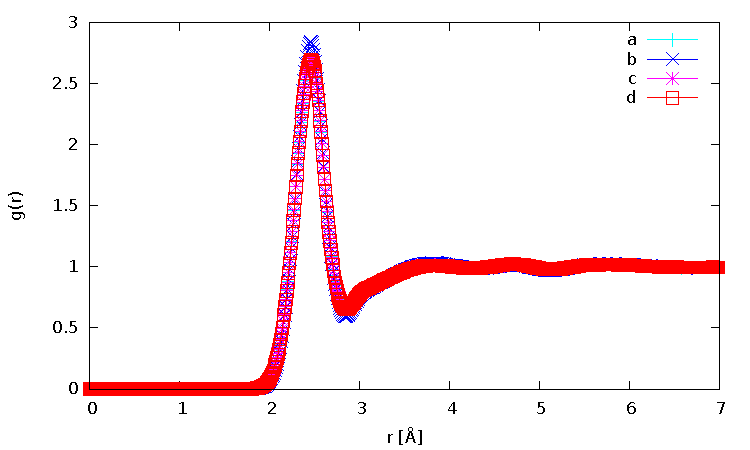
\includegraphics[width=0.475\textwidth]
{rdffixedpt.pdf}
\end{center}
\caption{\label{Fig1}
Pair correlation function for (a) liquid silicon (3000 K) and (b) liquid silicon with noisy forces introduced by different range of fixed point errors.
} \end{figure}

\begin{figure}[h!]%[!htpb,floatfix]
\begin{center}
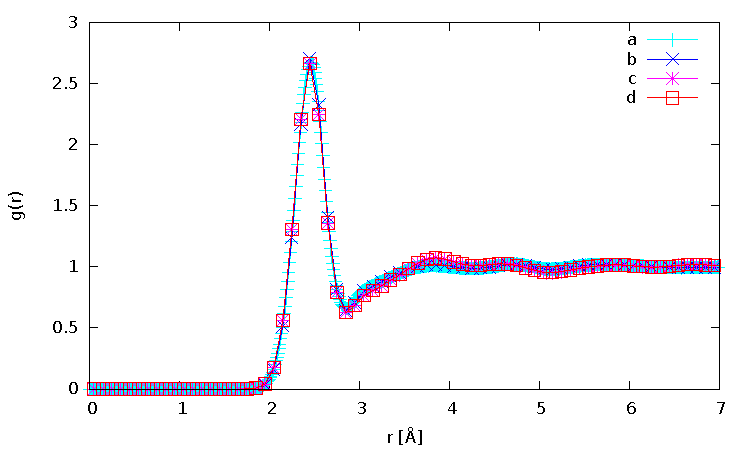
\includegraphics[width=0.475\textwidth]
{rdffloatingpt.pdf}
\end{center}
\caption{\label{Fig2}
Pair correlation function for (a) liquid silicon (3000 K) and (b) liquid silicon with noisy forces introduced by different range of floating point errors.
} \end{figure}

\begin{figure}[h!]%[!htpb,floatfix]
\begin{center}
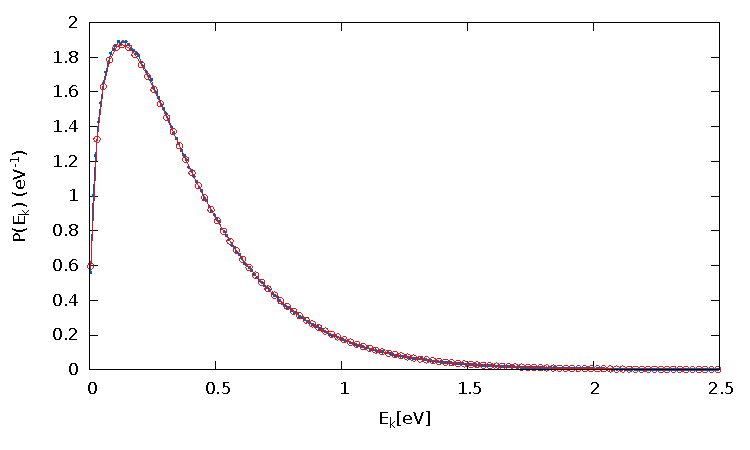
\includegraphics[width=0.475\textwidth]
{test1.pdf}
\end{center}
\caption{\label{Fig3}
Statistical properties in a 1000 atoms liquid Si simulation at 3000 K. (a) The ionic kinetic energy distributions (line) is compared with the exact Maxwell distribution (circles)
} \end{figure}

In Fig 3, the ionic kinetic energy distribution calculated with forces to which a computational error is added is compared with the exact Maxwell distribution line and it is seen that not only the average energy is correct but also its fluctuations follow the Maxwell distribution. 



\section{Summary}




\begin{acknowledgments}
The authors would like to thank the Gauss Center for Supercomputing (GCS) for providing computing time through the John von Neumann Institute for Computing (NIC) on the GCS share of the supercomputer JUQUEEN at the J\"ulich Supercomputing Centre (JSC). This project has received funding from the European Research Council (ERC) under the European Union's Horizon 2020 research and innovation programme (grant agreement No 716142).
\end{acknowledgments}

%\bibliography{paper}

\begin{thebibliography}{10}

%\bibitem{ball}
%P.~Ball,
%\newblock {\em Life's Matrix: A Biography of Water}
%\newblock (Univ of California Press 2001).
\bibitem{cp2kwebsite} 
CP2K Open Source Molecular Dynamics,
\\\texttt{http://cp2k.berlios.de}

\bibitem{bazantEIP} 
EIP Bazant potential,
\textit{tofill}

\bibitem{flyingIceCube} 
Stephen C. Harvey, Robert K.-Z. TAN, Thomas Cheatham. 
\textit{The Flying Ice Cube: Velocity Rescaling in Molecular Dynamics Leads to Violation of Energy Equipartition}

\bibitem{NumericalStabilityQC} 
Gerald Knizia, Wenbin Li, Sven Simon, Hans-Joachim Werner. 
\textit{Determining the Numerical Stability of Quantum Chemistry Algorithms}


\end{thebibliography}

%-----

\end{document}

